%
% brachistochrone.tex -- slide template
%
% (c) 2021 Prof Dr Andreas Müller, OST Ostschweizer Fachhochschule
%
\bgroup
\begin{frame}
\setlength{\abovedisplayskip}{5pt}
\setlength{\belowdisplayskip}{5pt}
\frametitle{Brachistochronenproblem}
%\vspace{-20pt}
\begin{columns}[t,onlytextwidth]
\begin{column}{0.64\textwidth}
\vspace*{-20pt}
\begin{center}
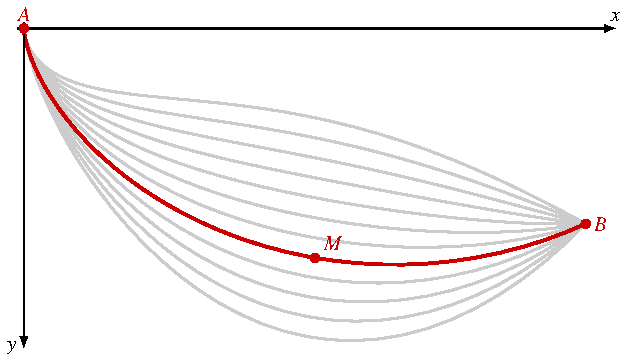
\includegraphics[width=0.96\textwidth]{../slides/2/bernoulli.pdf}
\end{center}
\end{column}
\begin{column}{0.36\textwidth}
Lagrange-Funktion:
\[
L(x,y,y')
=
\sqrt{
\frac{1+y^{\prime 2}}{y}
}
\]
Funktional zu minimieren:
\[
I(y) 
=
\int_{x_1}^{x_2}
\frac{\!\sqrt{1+y'(x)^2}}{\!\sqrt{y(x)}} \,dx
\]
Randbedingungen:
\[
y(x_1)=y_1
\quad\text{und}\quad
y(x_2)=y_2
\]
\end{column}
\end{columns}
\end{frame}
\egroup
